\renewcommand{\NomeBloco}{\textit{vref\_generator}}
\renewcommand{\NomeBlocoNoUnderline}{vrefgenerator}
\renewcommand{\NomePTab}{tab_\NomeBlocoNoUnderline}
\renewcommand{\NomeSTab}{tab_\NomeBlocoNoUnderline2}
\renewcommand{\NomePFig}{fig_\NomeBlocoNoUnderline}
\renewcommand{\NomeSFig}{fig_\NomeBlocoNoUnderline2}
\renewcommand{\NomeTTab}{tab_\NomeBlocoNoUnderline3}
\renewcommand{\NomeQTab}{tab_\NomeBlocoNoUnderline4}

\section{vref\_generator}

O \textit{\NomeBloco}\footnote{Circuito esquemático desenvolvido por \textit{Dalton Martini Colombo}} \'e o bloco respons\'avel por gerar todas as tensões de refer\^encia utilizados nos outros blocos do circuito. O bloco apresenta as definições de sinais de entrada e sa\'ida referidos na \autoref{\NomeSTab}.

\begin{table}[!h]
\caption{Sinais do bloco \NomeBloco}
\label{\NomeSTab}
\centering
\begin{tabular}{ccl}

    \toprule
    Sinal & Tipo    & Descrição      \\
    \midrule \midrule
    Ibias   & Entrada   & Corrente de polarização do bloco \textit{Par Diferencial} \\
    \midrule
    V\_extra   & Saída   & Tensão de refer\^encia de 1,15 V \\
    \midrule
    Vref\_plus   & Saída   & Tensão de refer\^encia de 1,02 V \\
    \midrule
    Vref   & Saída   & Tensão de refer\^encia de 898,45 mV \\
    \midrule
    y1   & Saída   & Tensão de refer\^encia de 772,67 mV \\
    \midrule
    y2   & Saída   & Tensão de refer\^encia de 646,89 mV \\
    \midrule
    y3   & Saída   & Tensão de refer\^encia de 521,1 mV \\
    \midrule
    y4  & Saída   & Tensão de refer\^encia de 395,32 mV  \\
    \midrule
    y5   & Saída   & Tensão de refer\^encia de 269,54 mV \\
    \midrule
    y6   & Saída   & Tensão de refer\^encia de 143,75 mV \\
    \bottomrule
\end{tabular}
\legend{Fonte: Produzido pelo autor}
\end{table}

O circuito projetado para o bloco \'e demonstrado na \autoref{\NomePFig}.

\begin{figure}[htb]
 \centering
    \centering
    \caption{\label{\NomePFig}Circuito CMOS projetado para o bloco \NomeBloco} 
    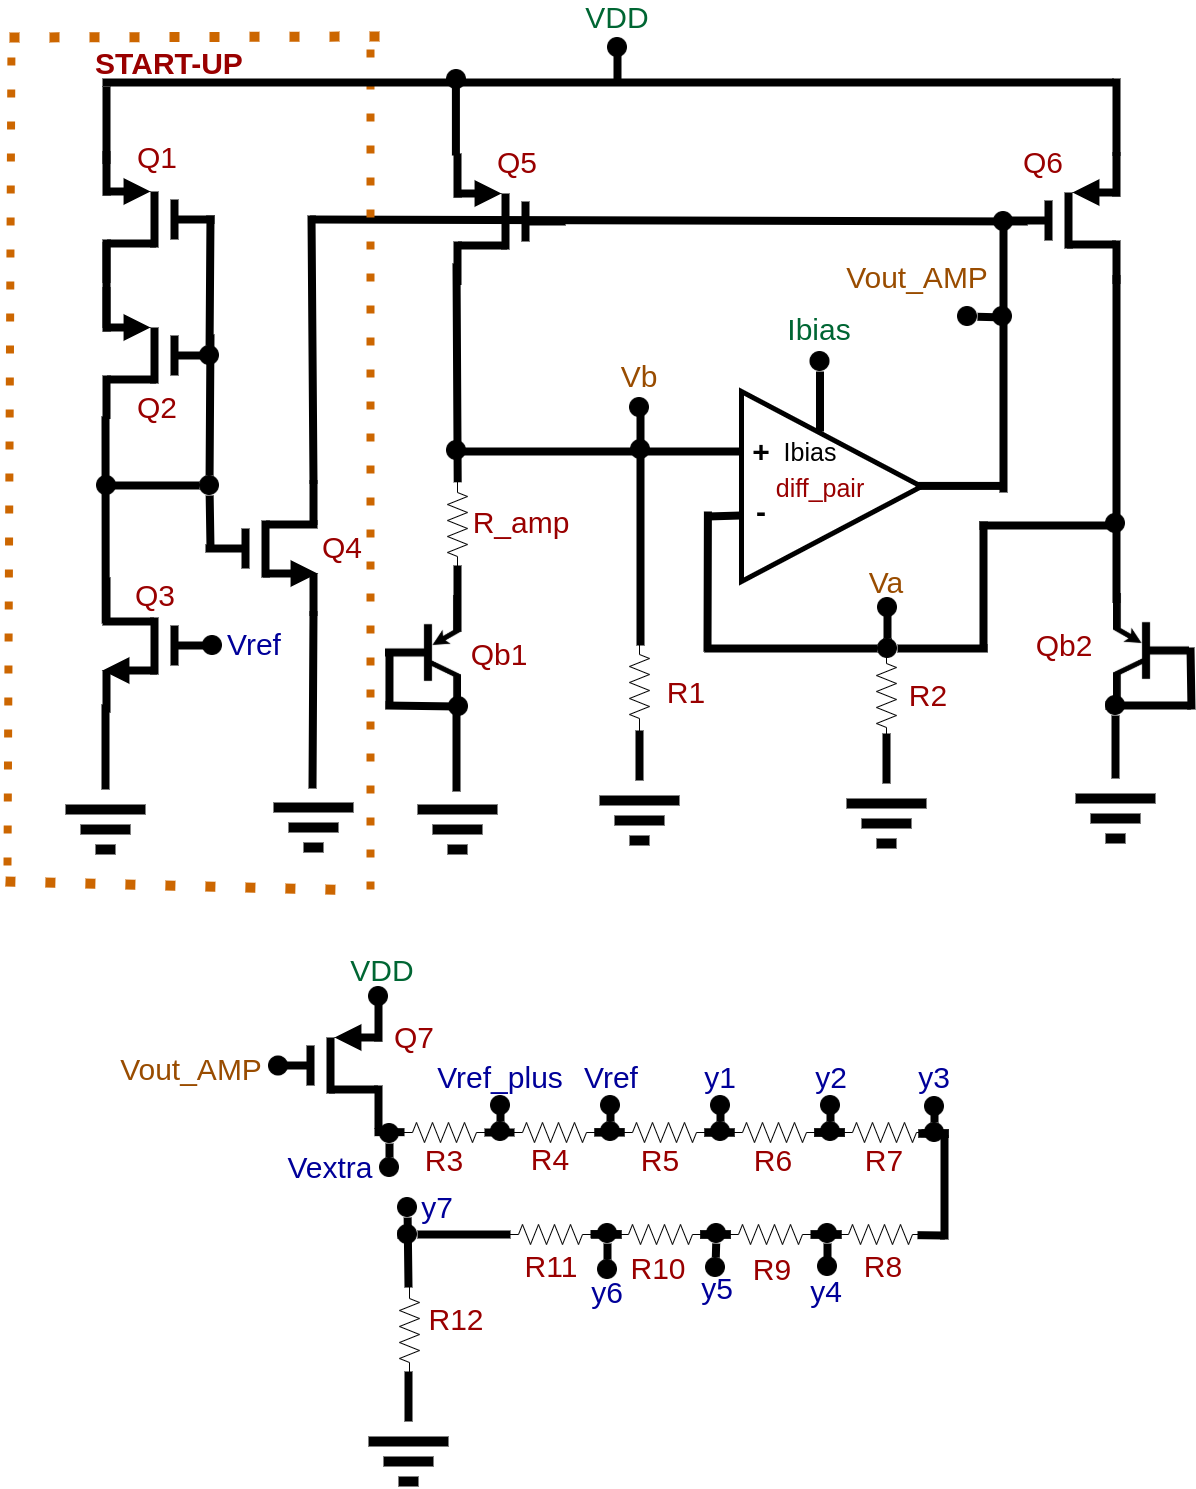
\includegraphics[scale=0.3]{Circuitos/vref_generator.png}
    \legend{Fonte: Produzido pelo autor}
\end{figure}

\begin{figure}[htb]
 \centering
    \centering
    \caption{\label{\NomeSFig}Representação em bloco do \NomeBloco}
    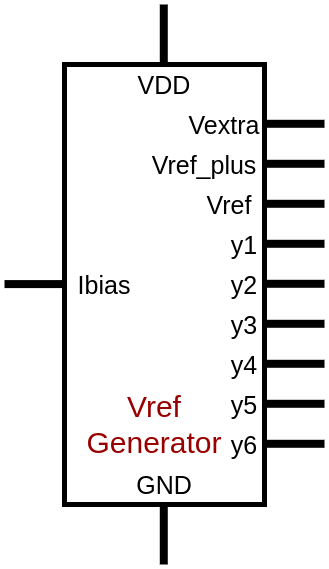
\includegraphics[scale=0.3]{Circuitos/vref_generator_block.png}
    \legend{Fonte: Produzido pelo autor}
\end{figure}

Os transistores utilizados no bloco \NomeBloco{} apresentam os par\^ametros mostrados na \autoref{\NomeTTab}.

\begin{table}[!h]
\caption{Transistores do Bloco \NomeBloco}
\label{\NomeTTab}
\centering
\begin{tabular}{ccccc}
\toprule
Transistor & W ($\mu$m)  & L ($\mu$m)           & M (n° dispositivos) & S (n° dispositivos)\\
\midrule \midrule
Q1 e Q2 & 0,5 & 19,995 & 1 & 1\\
\midrule
Q3 & 20 & 0,18 & 1 & 1\\
\midrule
Q4 & 2 & 0,18 & 1 & 1\\
\midrule
Q5, Q6 e Q7 & 20 & 16 & 4 & 1\\
\midrule
Qb1 (PNP) & 5 & 5 & 1 & 1\\
\midrule
Qb2 (PNP) & 5 & 5 & 8 & 1\\
\bottomrule
\end{tabular}
\legend{Fonte: Produzido pelo autor}
\end{table}

Os resistores utilizados no bloco \NomeBloco{} apresentam os par\^ametros mostrados na \autoref{\NomeQTab}.

\begin{table}[!h]
\caption{Resistores do bloco \NomeBloco}
\label{\NomeQTab}
\centering
\begin{tabular}{cccccc}
\toprule
Resistor & \begin{tabular}[c]{@{}c@{}}W \\($\mu$m)\end{tabular}   & \begin{tabular}[c]{@{}c@{}}L \\($\mu$m)\end{tabular}  & \begin{tabular}[c]{@{}c@{}}Resist\^encia\\ (k$\Omega$)\end{tabular} & \begin{tabular}[c]{@{}c@{}}M\\(n° dispositivos)\end{tabular} & \begin{tabular}[c]{@{}c@{}}S \\(n° dispositivos)\end{tabular}\\
\midrule \midrule
R1 e R2 & 2 & 18,85 & 10,1024 & 1 & 10\\
\midrule
\begin{tabular}[c]{@{}c@{}}R\_amp, R3, R4,\\ R5, R6, R7, \\ R8, R9, R10, \\ R11\end{tabular} & 2 & 18,85 & 10,1024 & 1 & 1\\
\midrule
R12 & 2 & 18,85 & 10,1024 & 7 & 1\\
\bottomrule
\end{tabular}
\legend{Fonte: Produzido pelo autor}
\end{table}

O dispositivo funciona produzindo uma corrente de refer\^encia extremamente est\'avel, utilizando um amplificador operacional e realimentação. O braço \textit{Q7} utiliza dessa corrente como refer\^encia para gerar uma corrente que alimenta alguns resistores, que geram os potenciais de refer\^encia desejados.
